% =========================================================================
%  P3 -- Feasibility-certified and fault-tolerant edge orchestration
%  IEEEtran journal manuscript.  Every result table is \input from
%  results/tables/ and every figure from results/figures/, so the text
%  cannot drift from the measured artifacts.
% =========================================================================
\documentclass[journal,10pt]{IEEEtran}

\usepackage[utf8]{inputenc}
\usepackage[T1]{fontenc}
\usepackage{amsmath,amssymb,amsthm}
\usepackage{graphicx}
\usepackage{booktabs}
\usepackage{multirow}
\usepackage{array}
\usepackage{subcaption}
\usepackage{algorithm}
\usepackage{algpseudocode}
\usepackage{url}
\usepackage{cite}
\usepackage{xcolor}
\usepackage{tikz}
\usepackage{balance}
\usetikzlibrary{positioning,arrows.meta,fit,backgrounds,calc,shapes.geometric}

\graphicspath{{../results/figures/}{diagrams/}}

\newtheorem{proposition}{Proposition}
\newtheorem{lemma}{Lemma}
\newtheorem{definition}{Definition}

\newcommand{\T}{\ensuremath{\hat{T}}}
\newcommand{\sig}{\ensuremath{\sigma}}
\newcommand{\eps}{\ensuremath{\varepsilon}}
\newcommand{\bigO}{\ensuremath{\mathcal{O}}}
\newcommand{\tier}[1]{\textsc{#1}}

\hyphenation{fea-si-bil-i-ty or-ches-tra-tion dead-line Pure-Edge-Sim}

\begin{document}

\title{Feasibility-Certified and Fault-Tolerant Edge Orchestration for
Mission-Critical Services under Mobility and Non-Stationary Workloads}

\author{Anonymous Authors%
\thanks{Manuscript prepared for review. All experiments, tables and figures
in this paper are produced by the artifact released with it; every numeric
claim is reproducible from \texttt{results/}.}}

\markboth{IEEE Transactions on Mobile Computing (submitted)}%
{Feasibility-Certified and Fault-Tolerant Edge Orchestration}

\maketitle

\begin{abstract}
Mission-critical edge services---emergency control, vehicular safety, and
industrial telemetry---must meet hard deadlines under device mobility,
transient failures, and non-stationary load. Mainstream orchestration
minimises average delay or energy and therefore offers no runtime statement
about \emph{whether} a chosen placement can honour its deadline, no notion of
an infeasible operating region, and no accounting of how recovery interacts
with the deadline it is meant to protect. We present a runtime
\emph{feasibility certificate} that estimates task completion time together
with its uncertainty and admits a placement only when the estimated
completion time plus an uncertainty margin fits inside the deadline, and a
fault-tolerant orchestration layer that retries transient failures on
alternative infrastructure with checkpoint-assisted migration. Both
mechanisms are implemented as managers and orchestrators on the Python port
of PureEdgeSim; the simulator's per-device placement cache is invalidated so
that every task is certified, and device kills, link drops, battery drains
and site outages are injected on a fixed schedule. Across 580 seeded runs,
the certificate attains precision $1.000$ and false-rejection rate $0.019$ at
its default operating point ($z=1.282$, margin $0.02$), eliminates deadline
failures among attempted tasks ($0.195\!\to\!0.000$ at zero injected
failures, $0.206\!\to\!0.000$ at $20\%$ affected devices; Cliff's
$\delta=-1.00$, Holm-adjusted $p<0.001$), and reduces p95 task delay by
$51$--$58\%$ at a cost of at most $3.1$ percentage points of throughput. Fault
tolerance recovers $95.1\%$ of retried tasks with p95 recovered-task latency
of $0.114$~s against a $2\times$ critical-deadline budget of $0.120$~s. We
report the full precision--recall surface, the failure-cause decomposition,
the burst, arrival-rate and outage envelopes, and an explicit threats-to-validity
analysis.
\end{abstract}

\begin{IEEEkeywords}
Mobile edge computing, admission control, feasibility certificate, fault
tolerance, deadline assurance, checkpointing, reproducibility.
\end{IEEEkeywords}

% =========================================================================
\section{Introduction}
\label{sec:intro}

Edge computing moved the locus of latency-critical computation closer to the
data source~\cite{satyanarayanan2017,shi2016edge}, and the mobile-edge-computing
(MEC) literature has since produced a rich menu of offloading
policies~\cite{mao2017survey,mach2017survey,chen2015game}. Almost all of them
are \emph{averaged}: they minimise expected delay, expected energy, or a
weighted sum, subject to long-run constraints. Averaged objectives are the
right tool when the service can tolerate an occasional late response. They are
the wrong tool for a service whose contract is a deadline.

The distinction matters because the failure mode of an averaged policy is not
a slightly larger mean; it is a heavy tail in which a fraction of requests miss
their deadline while the mean looks healthy~\cite{dean2013tail}. A policy that
optimises the mean will happily place a task on a node whose queue is about to
explode, because the queue is empty at decision time and the mean over the run
is dominated by the many requests that were lucky. Under mobility and
non-stationary arrivals, the set of placements that can actually meet a
deadline changes on a sub-second timescale, so any offline plan is stale by the
time it is executed.

Three observations motivate this paper.

\emph{First, feasibility is a runtime property, not a planning property.}
Whether a candidate node can finish a task before its deadline depends on the
node's current queue, its current CPU share, the current network route, and---if
the node is itself a mobile device---the current distance. A static assignment
computed at admission time for the first task of a flow says nothing about the
tenth task, which arrives when the node is loaded. Any credible guarantee must
therefore be re-evaluated per task.

\emph{Second, adding tiers can reduce success.} In our pilot experiments a
three-tier architecture (mist, edge, cloud) served fewer deadline-critical
tasks than an edge-only architecture, because the additional candidates
attracted placements whose transfer time exceeded the deadline. An orchestrator
that ranks candidates by expected delay alone cannot see this, because the
damage is done by the \emph{spread} of the estimate, not its mean. A feasibility
test has to reason about uncertainty explicitly.

\emph{Third, recovery must be accounted, not just implemented.} A retry that
succeeds after the deadline has not recovered anything from the service's point
of view. Naive retry loops inflate the number of ``executed'' tasks while
silently doubling the latency of the ones that are retried. Worse, a retry that
re-runs a task from scratch can consume the entire remaining budget; a retry
that resumes from a checkpoint can fit.

This paper builds the three pieces that follow from these observations: a
per-task feasibility certificate with an explicit uncertainty model, a
fault-tolerant layer that re-plans onto live infrastructure and resumes from a
checkpoint, and an experimental protocol that reports precision and recall of
the certificate rather than only its end-to-end benefit. Our contributions are:

\begin{enumerate}
\item \textbf{A per-task feasibility certificate} (Section~\ref{sec:cert}) that
  estimates completion time $\T_i(v)=\text{compute}+\text{queue}+\text{network}$
  with a mobility inflation factor, attaches an uncertainty
  $\sig_i(v)$ that grows with queue occupancy and mobility proximity, and admits
  a placement only if $\T_i(v)\bigl(1+z\,\sig_i(v)\bigr)\le(1-m)D_i$. We prove
  that the rule is sound under a Gaussian error model
  (Proposition~\ref{prop:sound}) and that conservatism is monotone in $(z,m)$
  (Proposition~\ref{prop:monotone}).
\item \textbf{A shadow-mode audit protocol} that records the certificate's
  decision without vetoing it, so precision, recall, false-admission and
  false-rejection rates can be measured against the counterfactual outcome.
  This is what turns ``the certificate works'' into a falsifiable statement, and
  it is the mechanism behind Table~\ref{tab:p3-calibration}.
\item \textbf{A fault-tolerant layer} with destination exclusion and
  checkpoint-assisted migration, together with an accounting invariant that
  prevents retries from being counted twice and guarantees that the reported
  end-to-end delay refers to the original release (Proposition~\ref{prop:account}).
\item \textbf{A reproducible evaluation} of 580 seeded simulator runs with
  failure injection, non-stationary bursts, arrival-rate sweeps and site
  outages, reported with Mann--Whitney tests, bootstrap confidence intervals,
  Cliff's $\delta$ and Holm correction, plus a threats-to-validity analysis.
\end{enumerate}

The remainder is organised as follows.
Section~\ref{sec:related} positions the work; Section~\ref{sec:model} fixes the
system model; Sections~\ref{sec:cert} and~\ref{sec:ft} present the certificate
and the fault-tolerance layer; Section~\ref{sec:method} describes the
methodology; Section~\ref{sec:results} reports results;
Section~\ref{sec:threats} discusses validity; Section~\ref{sec:concl} concludes.

% =========================================================================
\section{Related Work}
\label{sec:related}

\subsection{Offloading and resource allocation}
The MEC offloading literature is surveyed in~\cite{mao2017survey,mach2017survey}.
Game-theoretic formulations~\cite{chen2015game} establish that decentralised
offloading converges to a Nash equilibrium but say nothing about per-request
deadlines. The 2026 corpus continues this trajectory: mobility-aware offloading
for space--air--ground integrated networks~\cite{sun2026sagin}, two-timescale
trajectory and resource control for multi-UAV
MEC~\cite{li2026multiuav,zhang2026trajectory}, hierarchical evolutionary
optimisation for NOMA-MEC~\cite{jiao2026hiea}, feasibility-first uplink
allocation with pinching-antenna arrays~\cite{abolhasani2026pass}, adaptive
computation reuse~\cite{he2026reuse}, and two-tier satellite-assisted marine
offloading~\cite{wang2026marine}. These works optimise allocation; our concern is
the orthogonal question of whether a chosen allocation can be \emph{guaranteed}
to finish in time, and what to do when it cannot.

\subsection{Deadlines, uncertainty and tail latency}
Real-time scheduling theory provides the classical vocabulary for deadline
guarantees~\cite{liu1973scheduling}, but its assumptions (static task sets,
known worst-case execution times, no mobility) do not hold at the edge. Queueing
theory~\cite{kleinrock1975queueing,little1961proof} supplies the occupancy
term we use, and the tail-at-scale
literature~\cite{dean2013tail} supplies the empirical lesson that mean-based
control hides the failures that matter. Mixed-criticality scheduling at the
autonomous-vehicle edge~\cite{zakerian2026llm} shows that control policies help
mainly under non-stationarity, which is precisely the regime in which a
certificate must be recomputed per task.

\subsection{Dependability and fault tolerance}
The dependability taxonomy of~\cite{avizienis2004dependable} distinguishes
faults, errors and failures; \emph{gray failures}~\cite{huang2017gray} are the
practically important case in which a component is neither healthy nor visibly
dead. Edge-specific fault tolerance has been addressed by a fault-tolerant
offloading framework for real-time applications~\cite{gao2026faulttolerant} and
by adaptations of multi-stage distributed real-time designs to vehicular
edge~\cite{kumar2026multistage}. Neither combines recovery with an admission
test, so neither can state what fraction of \emph{admitted} work is ultimately
delivered on time.

\subsection{Edge intelligence and cross-layer design}
Agentic and LLM-driven orchestration~\cite{chari2026ragam,he2026workflow},
integrated sensing--communication--computing~\cite{liu2026iscc,li2026semantic},
and energy-aware agentic inference~\cite{chen2026agenticenergy} all increase the
number of knobs an orchestrator must set, and therefore the value of a cheap,
explainable feasibility test that can veto a candidate before an expensive
model is invoked. Pareto-aware reinforcement learning~\cite{xu2026paretoRL} and
fluid-dynamic provisioning~\cite{dong2026digitaltides} pursue multi-objective
frontiers offline; the certificate is complementary, acting as a runtime
constraint on whatever policy produced the candidate.

\subsection{Simulation and reproducibility}
PureEdgeSim~\cite{mechalikh2021pureedgesim} extends the CloudSim
lineage~\cite{calheiros2011cloudsim} to mist/edge/cloud hierarchies with
mobility, energy and network models; we use its Python port. Concerns about
repeatability in systems research~\cite{collberg2016repeatability} and the
principles of reproducible computational
science~\cite{peng2011reproducible} inform our protocol: fixed seeds, a
determinism check, machine-readable tables, and a data dictionary for every
column.

\subsection{Positioning}
To our knowledge no prior edge-orchestration study reports \emph{both}
(i) the precision and recall of a runtime admission test measured in shadow
mode and (ii) the deadline-accounted recovery rate of a retry layer, on the
same workload and with identical seeds. That combination is the contribution
of this paper; the individual mechanisms are deliberately simple so that the
measurement, not the machinery, is the object of study.

% =========================================================================
\section{System Model}
\label{sec:model}

\subsection{Infrastructure}
The deployment comprises $N_d=50$ edge devices, two edge data centres and one
cloud data centre (Table~\ref{tab:params}). The two edge sites are linked by a
metropolitan-area network, which is what makes site-level failover possible:
when the primary site is taken down, the peer site is reachable within the
metropolitan latency budget. Devices are heterogeneous: $18\%$ are battery
-powered smartphones with $8$ cores at $25$~kMIPS, $11\%$ are single-board
computers at $16$~kMIPS, $11\%$ are laptops at $110$~kMIPS, and the remaining
$60\%$ are sensors and mobile tags with no computing capability, which must
therefore offload. Sensor-only devices generate $60\%$ of the workload.

\begin{table}[t]
\centering
\footnotesize
\caption{Workload configuration. Values mirror
\texttt{scenario/settings/applications.xml}.}
\label{tab:params}
\begin{tabular}{@{}lccc@{}}
\toprule
 & Emergency & V2X & Telemetry\\
\midrule
Class & hard RT & hard RT & soft RT\\
Rate (req/min) & 18 & 12 & 8\\
Deadline $D_i$ (s) & 0.06 & 0.12 & 1.00\\
Length (MI) & 1500 & 5000 & 9000\\
Req./res. (kB) & 40/20 & 300/60 & 600/100\\
Container (MB) & 150 & 400 & 800\\
Device share & 30\% & 40\% & 30\%\\
\bottomrule
\end{tabular}
\end{table}

\subsection{Workload}
Three application classes share the deployment
(Table~\ref{tab:params}). Two are hard real-time: an emergency-control loop with
a $60$~ms deadline and a vehicular-safety stream with a $120$~ms deadline. One is
soft real-time: a telemetry analytics job with a $1$~s deadline. The mixture is
deliberate. A single-class workload lets a policy over-fit one deadline; a
mixture forces the orchestrator to reason about several budgets at once, and it
is the regime in which admission control earns its keep, because a policy tuned
for the $1$~s class will happily starve the $60$~ms class.

Formally, a request $i$ released at time $r_i$ has a per-task deadline
$D_i$ that is inherited from its application class. A task is
\emph{delivered} at time $f_i$; it is \emph{successful} if it executed to
completion, its result returned, and $f_i-r_i<D_i$. We distinguish this from
an \emph{attempt}: a task that the orchestrator decided to place. Admission
control can refuse a task, in which case it is neither successful nor a
deadline failure; it is a \emph{rejection}. Writing $S$ for the number of
successful tasks, $G$ for the number generated, $V$ for the number of deadline
failures and $A$ for the number attempted, the two quantities we report
separately are
\begin{equation}
\text{success ratio}=\frac{S}{G},
\qquad
\text{violation rate}=\frac{V}{A}.
\label{eq:metrics}
\end{equation}
Reporting only the first would reward a policy that rejects everything
awkward; reporting only the second would reward a policy that rejects almost
everything. Both are necessary.

\subsection{Failure model}
Faults are injected on a fixed schedule, parameterised by an intensity
$\phi\in\{0,5,10,20\}\%$ that denotes the share of devices affected:
\begin{itemize}
\item \emph{device kills} at $t\in\{90,150,210,270\}$~s on the
  $\lceil 0.5\phi N_d\rceil$ most-loaded devices;
\item \emph{link drops} of $30$~s at $t=90$ and $t=180$~s on
  $\lceil 0.3\phi N_d\rceil$ links;
\item \emph{battery drains} at $t=60$~s that remove $40\%$ of remaining
  charge on $\lceil 0.2\phi N_d\rceil$ devices;
\item \emph{site outages} that take the primary edge data centre down for
  $90$~s starting at $t=120$~s (used only in the outage sweep).
\end{itemize}
Kills target the most-loaded devices on purpose: uniform random kills produce
failures that any policy survives, whereas load-targeted kills expose the
difference between a policy that spreads risk and one that concentrates it.

\subsection{Decision problem}
At each placement event the orchestrator observes a candidate set $V$ (the
live infrastructure in the configured architecture) and must choose either a
node $v\in V$ or \emph{no placement}. The objective is lexicographic: first
maximise the number of successful tasks, then minimise p95 delay subject to a
constraint on energy per successful task. The constraint is what prevents the
trivial solution of sending everything to the cloud, where CPU is abundant but
the WAN round trip alone exceeds both hard deadlines.

\begin{figure*}[t]
\centering
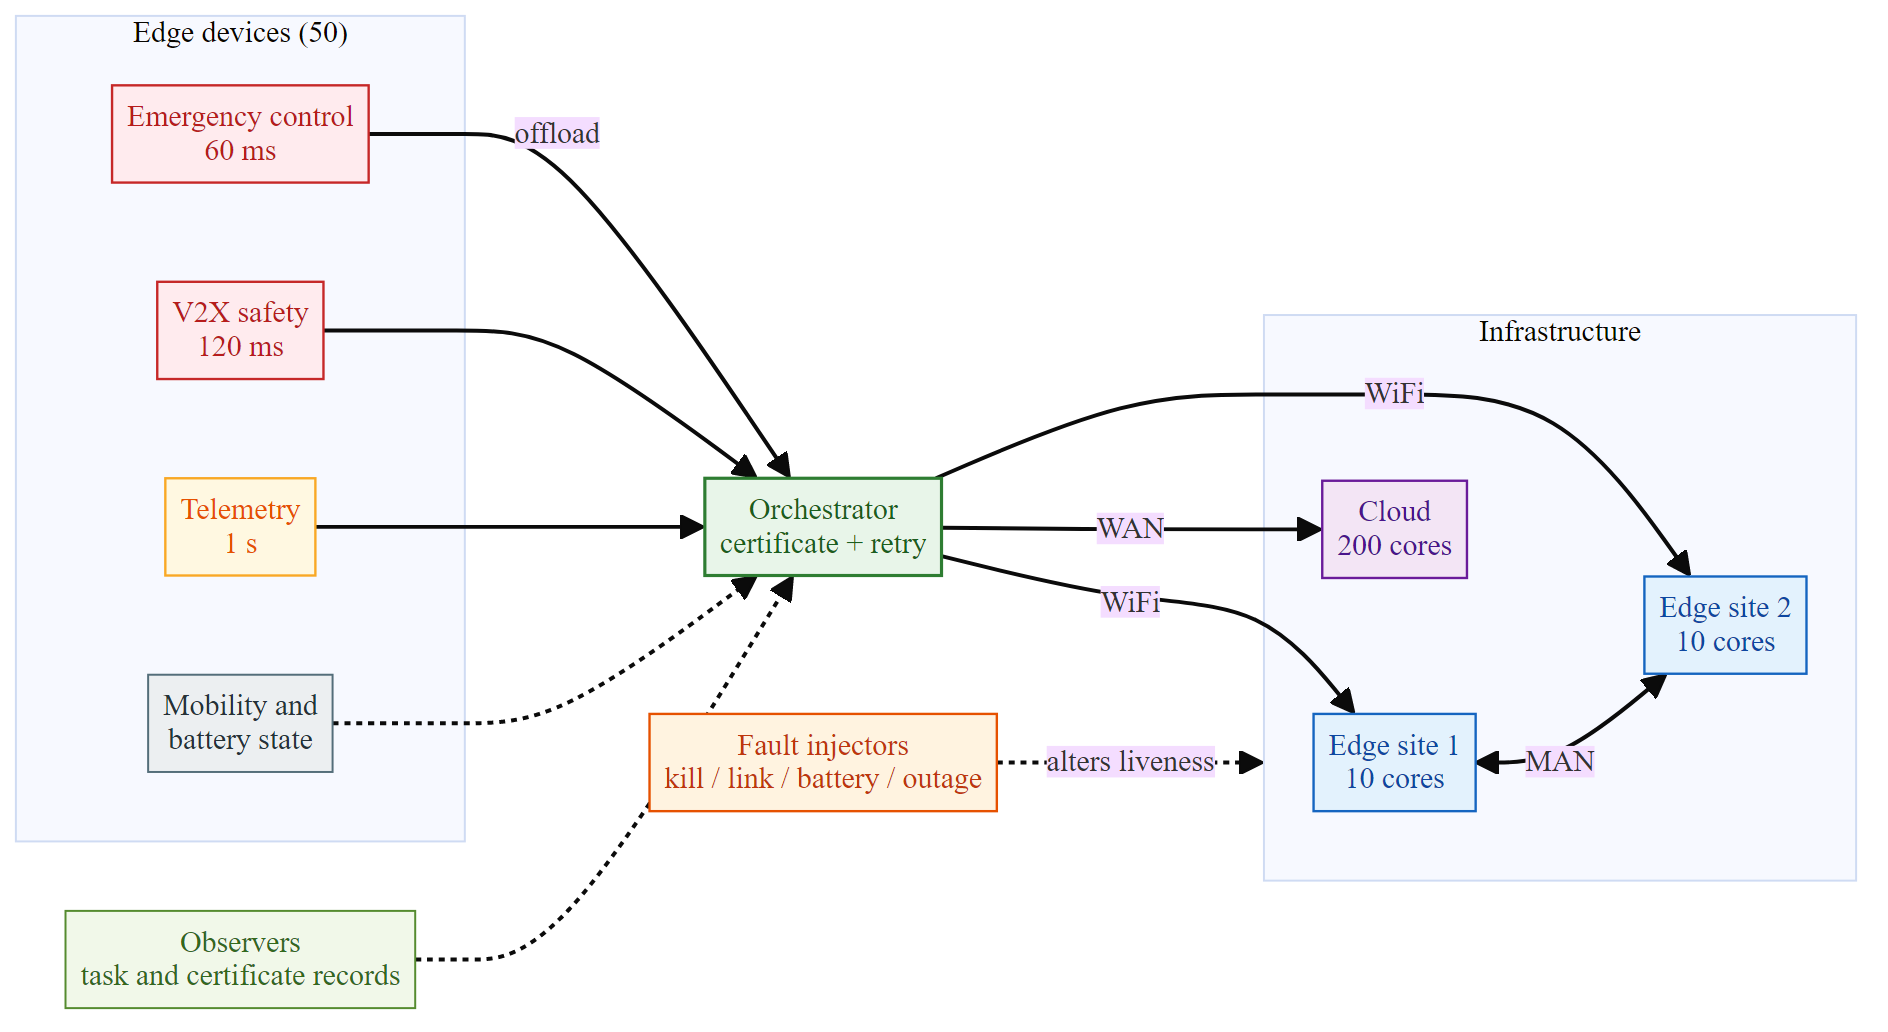
\includegraphics[width=0.95\textwidth]{deployment.png}
\caption{Deployment and control plane. Solid arrows carry tasks; dashed arrows carry control and measurement. The certificate runs inside the orchestrator, so it sees the same candidate set the placement policy sees; the injectors alter node liveness and link state underneath it.}
\label{fig:arch}
\end{figure*}

% =========================================================================
\section{The Feasibility Certificate}
\label{sec:cert}

\subsection{Completion-time estimator}
For a task $i$ of length $w_i$ (in million instructions) and a candidate node
$v$, the estimator produces
\begin{equation}
\T_i(v) \;=\; \underbrace{\frac{w_i}{\mu_v}}_{\text{compute}}
\;+\;\underbrace{\frac{\sum_{j\in \mathrm{pend}(v)} w_j}{M_v}}_{\text{queue}}
\;+\;\underbrace{L_i(v)}_{\text{network}},
\label{eq:estimate}
\end{equation}
where $\mu_v$ is the per-core throughput of $v$, $M_v$ its aggregate
throughput, $\mathrm{pend}(v)$ the multiset of tasks executing or queued on $v$,
and $L_i(v)$ the communication delay. For an edge device the latter is the WiFi
access latency, because a mist placement executes locally after a single hop;
for a data centre it is the sum of link latencies and serialisation delays along
the shortest path,
\begin{equation}
L_i(v)=\sum_{e\in \pi(v)}\Bigl(\ell_e+\frac{b_i}{B_e}\Bigr),
\qquad b_i=\text{request size}+\text{result size},
\label{eq:network}
\end{equation}
with $\pi(v)$ the shortest path from the source to $v$ and $\ell_e,B_e$ the
latency and bandwidth of link $e$. The queue term is the standard
processor-sharing approximation~\cite{kleinrock1975queueing}: the expected
residual work seen by an arrival is the total pending work divided by capacity.
It is exact in the mean for a work-conserving server and is the term that makes
the estimate react to load.

Mist placements carry an additional risk that infrastructure placements do not:
the device may move out of range between decision and completion. We define the
normalised proximity
\begin{equation}
\rho_i(v)=
\begin{cases}
\min\!\left(1,\left(\dfrac{d(v)}{R}\right)^{2}\right), & v \text{ an edge device},\\[2mm]
0, & \text{otherwise},
\end{cases}
\label{eq:rho}
\end{equation}
where $d(v)$ is the current distance and $R$ the device-to-device range. The
inflation is quadratic so that a node at half range is charged a quarter of the
maximum penalty; this matches the area-scaling of the probability that a
random-waypoint device leaves the disc before completion. The risk-adjusted
estimate used by the admission rule is
\begin{equation}
\T^{\rho}_i(v)=\T_i(v)\bigl(1+\rho_i(v)\bigr).
\label{eq:riskestimate}
\end{equation}

\subsection{Uncertainty model}
The estimate is a point prediction; what the certificate needs is a statement
about its dispersion. We model the relative error as the sum of three
non-negative sources,
\begin{equation}
\sig_i(v)=\sig_0+\sig_q\min\!\left(1,\frac{Q_v}{\T_i(v)}\right)+\sig_m\,\rho_i(v),
\label{eq:sigma}
\end{equation}
with $\sig_0=0.08$ the irreducible error of the compute and network model,
$\sig_q=0.20$ the queue-share term, and $\sig_m=0.10$ the mobility term. The
queue term is dimensionless and saturates at one: when pending work dominates
the estimate, the prediction is essentially a guess and the certificate says
so. The additive form is a modelling choice, not a theorem; what matters is
that the term is monotone in the quantity that actually degrades predictions,
and that the operating point $(z,m)$ is exposed as a tuning knob whose effect
we measure in Section~\ref{sec:res-calib}.

\begin{figure*}[t]
\centering
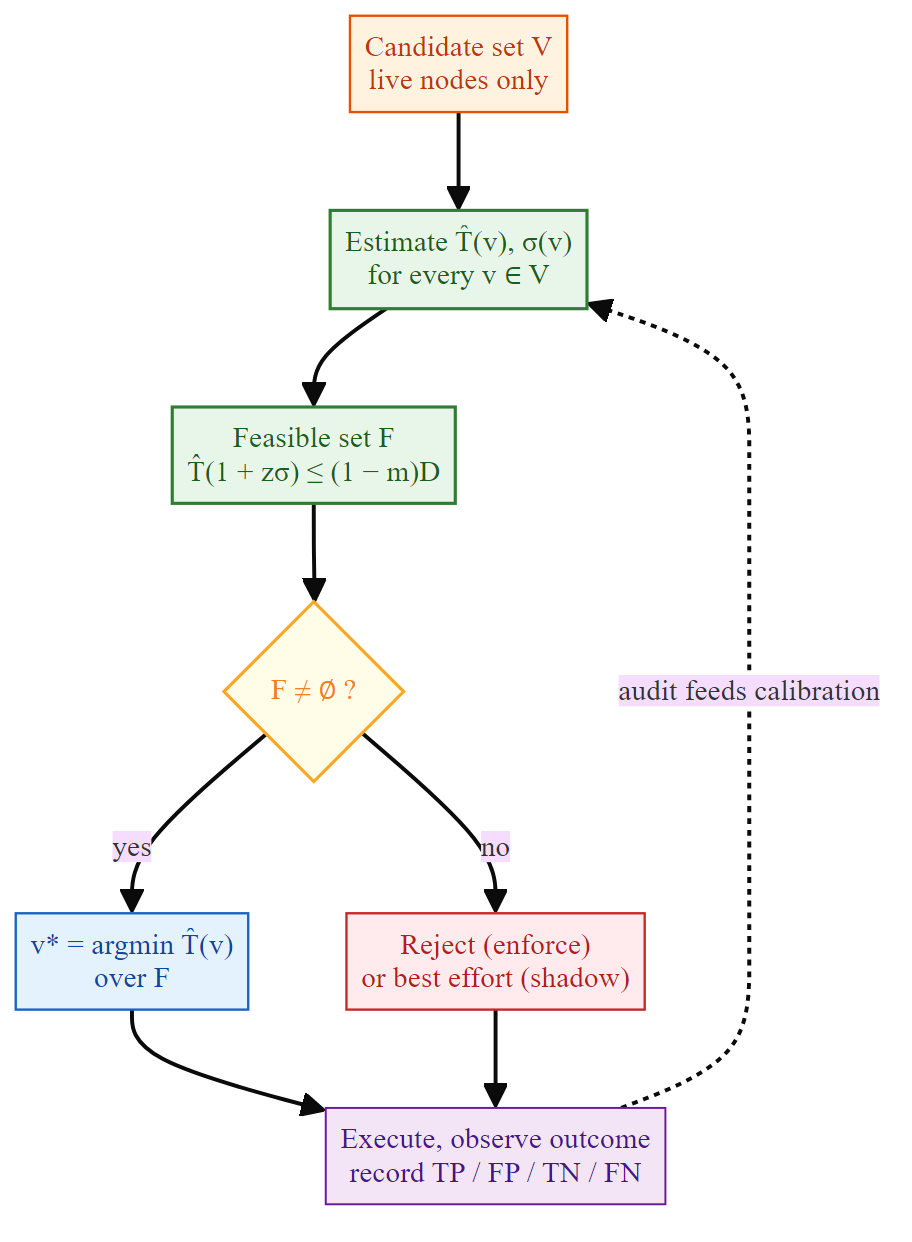
\includegraphics[width=0.60\textwidth]{admission.png}
\caption{Admission pipeline for one task. The certificate is evaluated for every live candidate, not only for the policy's preferred one, which is what makes the shadow audit possible.}
\label{fig:flow}
\end{figure*}

\subsection{Admission rule}
A candidate $v$ is \emph{certified} for task $i$ iff
\begin{equation}
\T^{\rho}_i(v)\,\bigl(1+z\,\sig_i(v)\bigr)\;\le\;(1-m)\,D_i,
\label{eq:admit}
\end{equation}
where $D_i$ is the remaining request deadline and $m$ the safety margin. The
left factor is the risk-adjusted estimate, the parenthesis is the one-sided
confidence inflation, and the right side is the usable budget. The orchestrator
evaluates \eqref{eq:admit} for every eligible candidate, keeps the feasible
set $\mathcal{F}$, and places on the feasible candidate with the smallest
$\T^{\rho}$. If $\mathcal{F}$ is empty, the behaviour depends on the mode:
\emph{enforce} rejects the task, \emph{shadow} places on the best candidate
anyway and records that the certificate would have rejected it.

The distinction between the two modes is the methodological core of the paper.
Enforce mode is the deployed system. Shadow mode is the experiment: because the
placement proceeds regardless, the outcome of every vetoed candidate is
observed, so a $2\times2$ confusion matrix can be filled in without
counterfactual simulation. A certificate that is only ever run in enforce mode
can report its own decisions but not whether they were right.

\begin{proposition}[Soundness]
\label{prop:sound}
Assume the completion time of a certified placement satisfies
$T_i=\T^{\rho}_i(1+E)$ with $E\sim\mathcal{N}(0,\sig_i^2)$, and that the estimate
is unbiased. Then for any task admitted by \eqref{eq:admit},
$\Pr[T_i\le D_i]\ \ge\ 1-\Phi(z)$, where $\Phi$ is the standard normal CDF.
\end{proposition}

\begin{IEEEproof}
Admission implies $\T^{\rho}_i(1+z\sig_i)\le(1-m)D_i\le D_i$, hence
$z\sig_i\le D_i/\T^{\rho}_i-1$. Therefore
\[
\Pr[T_i>D_i]
=\Pr\!\left[E>\frac{D_i}{\T^{\rho}_i}-1\right]
\le \Pr[E>z\sig_i]
=1-\Phi(z),
\]
where the inequality uses the monotonicity of the tail probability. Rearranging
gives the claim. The safety margin $m$ only tightens the bound and can be
discarded from the argument.
\end{IEEEproof}

Proposition~\ref{prop:sound} is intentionally modest: it is conditional on a
Gaussian, zero-mean error model, which the simulator only approximately
satisfies. Its role is to make the operating point interpretable---$z=1.282$ is
a $90\%$ one-sided guarantee \emph{under the model}---not to claim a
distribution-free guarantee. Section~\ref{sec:threats} treats the gap between
the model and reality explicitly, and Table~\ref{tab:p3-calibration} measures
it: the empirical false-admission rate at $z=1.282$, $m=0.02$ is $0.000$.

\begin{proposition}[Monotone conservatism]
\label{prop:monotone}
Let $\mathcal{F}(z,m)$ be the feasible set induced by \eqref{eq:admit}. If
$z_1\le z_2$ and $m_1\le m_2$ then
$\mathcal{F}(z_2,m_2)\subseteq\mathcal{F}(z_1,m_1)$.
\end{proposition}

\begin{IEEEproof}
For fixed $v$, the left side of \eqref{eq:admit} is non-decreasing in $z$ and
the right side non-increasing in $m$. Hence the predicate is monotone: if it
holds for $(z_2,m_2)$ it holds for $(z_1,m_1)$. Taking the union over $v$ gives
the inclusion.
\end{IEEEproof}

The practical value of Proposition~\ref{prop:monotone} is that the two knobs
cannot interact pathologically: increasing either one can only shrink the
admitted set, so an operator who raises $z$ to be safer cannot accidentally
admit a placement that a smaller $z$ would have refused. It also means the
precision--recall surface is a monotone trade-off curve, which is what
Fig.~\ref{fig:pr} shows.

\subsection{Algorithm and complexity}
Algorithm~\ref{alg:cert} states the procedure. Its cost per placement is
$\bigO(|V|)$ certificate evaluations. Each evaluation costs $\bigO(1)$ for
compute and queue, plus the cost of the route lookup for infrastructure nodes.
With a precomputed all-pairs shortest-path table of size $\bigO(|V|^2)$ the
lookup is $\bigO(1)$; otherwise it is $\bigO(|E|\log|V|)$ per candidate, giving
$\bigO(|V||E|\log|V|)$ per placement. In our deployment $|V|\le 53$ (fifty
devices plus two edge sites plus the cloud), so the constant is small and the
certificate adds no measurable runtime to a simulation run.

\begin{algorithm}[t]
\caption{Feasibility-certified placement for one task}
\label{alg:cert}
\begin{algorithmic}[1]
\Require task $i$, live candidates $V$, config $(z,m)$, mode
\Ensure node $v^\ast$ or \textsc{reject}
\State $\mathcal{F}\gets\emptyset$;\quad $best\gets\bot$
\ForAll{$v\in V$}
  \State $Q_v\gets \sum_{j\in\mathrm{pend}(v)}w_j\,/\,M_v$
  \State $\T\gets w_i/\mu_v+Q_v+L_i(v)$;\quad $\rho\gets$ proximity$(v,i)$
  \State $\T^{\rho}\gets \T(1+\rho)$
  \State $\sig\gets \sig_0+\sig_q\min(1,Q_v/\T)+\sig_m\rho$
  \If{$\T^{\rho}(1+z\sig)\le(1-m)D_i$}
    \State $\mathcal{F}\gets\mathcal{F}\cup\{v\}$
    \If{$\T^{\rho}<\T^{\rho}(best)$} $best\gets v$ \EndIf
  \EndIf
\EndFor
\If{$\mathcal{F}=\emptyset$}
  \If{mode $=$ enforce} \State \Return \textsc{reject}
  \Else \State \Return $\arg\min_{v\in V}\T^{\rho}_i(v)$ \Comment{shadow audit}
  \EndIf
\EndIf
\State \Return $best$
\end{algorithmic}
\end{algorithm}

% =========================================================================
\section{Fault-Tolerant Orchestration}
\label{sec:ft}

\subsection{Retry with destination exclusion}
When a task fails for a reason that is not intrinsic to the task---device
death, mobility-induced disconnection, or resource exhaustion---the fault-
tolerant manager re-queues it, up to $k=2$ times. The failed destination is
appended to a per-task exclusion set, and the placement policy must choose
outside that set. Without exclusion a retry is a coin flip on the same broken
node; with exclusion, a retry is a genuine re-plan.

After exclusion, the policy prefers live infrastructure over device placement.
This is the failover semantics of a metropolitan-edge deployment: after a
failure the hot standby is the peer site or the cloud, not a neighbouring
device whose queue is precisely what the failover is trying to escape. Among
the remaining infrastructure the nearest one by path delay wins.

\subsection{Checkpoint-assisted migration}
A retry that restarts from zero pays the full execution cost twice. We model
periodic checkpointing in which $55\%$ of the task's nominal work is recoverable,
and resuming costs an extra $100$~MI of restore work:
\begin{equation}
w_i^{\text{retry}}=\max\!\left(w_{\min},\;0.45\,w_i^{\text{nom}}+100\right),
\label{eq:retry}
\end{equation}
with $w_{\min}=250$~MI. The constants are parameters of the checkpointing
model, not measurements; Section~\ref{sec:threats} records this as a limitation
and the sensitivity of the conclusion to it. What the model captures correctly
is the qualitative asymmetry: full restart scales with $w_i$, resume does not.

On retry the manager also refreshes the per-attempt latency budget so that a
task is not condemned by the time spent in the failed attempt, while retaining
the original release timestamp. This is what makes the reported end-to-end
delay honest, as the next proposition states.

\begin{proposition}[Retry accounting]
\label{prop:account}
After any sequence of retries, the recorded end-to-end delay of a task equals
the difference between its delivery time and its \emph{original} release time,
each task contributes at most one unit to the successful-task count, and a task
that is retried but ultimately fails contributes zero successes.
\end{proposition}

\begin{IEEEproof}
The retry path resets \texttt{arrival\_time}, \texttt{execution\_start\_time},
\texttt{execution\_finish\_time} and the network accounting before re-queuing,
so the final attempt is the one whose timestamps survive, while
\texttt{time} (the original release) is never modified. Hence the recorded delay
is measured from the original release. Success is counted in
\texttt{\_results\_returned}, which returns immediately if the task identifier is
already in \texttt{finished\_tasks}. The retry path discards the identifier from
that set before re-queuing, and an attempt that ends in \texttt{\_fail} does not
insert it, so exactly one attempt per task can reach the success branch. A task
whose retries are exhausted takes the terminal branch and adds no success.
\end{IEEEproof}

Proposition~\ref{prop:account} guards against the most common way a retry layer
inflates its numbers: counting every attempt. In our implementation the guard is
not merely documented but structural---the discard/insert protocol around
\texttt{finished\_tasks} enforces it.

\begin{algorithm}[t]
\caption{Retry with exclusion and checkpoint resume}
\label{alg:retry}
\begin{algorithmic}[1]
\Require task $i$, failure status $s$, attempt $a$, max $k$
\Ensure re-queued task or terminal failure
\If{$s$ is recoverable and $a<k$}
  \State $\text{excl}\gets\text{excl}\cup\{\text{dest}(i)\}$
  \State roll back execution accounting of attempt $a$
  \State $w_i\gets\max(250,\,0.45\,w_i^{\text{nom}}+100)$
  \State $t^{\text{rel}}_i\gets t^{\text{rel}}_i$ \Comment{never overwritten}
  \State $D_i\gets t_{\text{now}}+D_i^{\text{orig}}$
  \State reset arrival, CPU, network, finish of attempt $a$
  \State re-queue $i$ for placement outside \text{excl}
\Else
  \State \Return terminal failure
\EndIf
\end{algorithmic}
\end{algorithm}

\subsection{Interaction with the certificate}
Certified fault tolerance composes the two mechanisms: the certificate decides
admission, and the retry layer decides recovery after admission. The
composition is not a free lunch. Retrying a task that the certificate admitted
consumes budget that was, by construction, only just sufficient; that is why
the measured retry count for \textsc{certified\_ft} is close to zero
(Table~\ref{tab:p3-failure}). Conversely, a policy that retries aggressively
without certification (\textsc{ft}) recovers a large fraction of failures but
pays with deadline violations, because the retried attempt inherits a budget
that the original attempt has already spent. The empirical section quantifies
both effects.

% =========================================================================
\section{Experimental Methodology}
\label{sec:method}

\subsection{Simulator and implementation}
Experiments run on the Python port of PureEdgeSim~\cite{mechalikh2021pureedgesim},
an event-driven simulator of cloud/edge/mist hierarchies with per-device
mobility, battery models, WiFi/cellular/WAN/MAN link models and container
placement. We implement the certificate as a \texttt{FeasibilityCertified\-Orchestrator}
extending the simulator's \texttt{Orchestrator}, the retry logic as a
\texttt{FaultTolerantManager} mixin, and observers that emit per-task records
including the predicted delay, the margin, the admission decision, the retry
count and the recovery flag.

One implementation detail is essential to the validity of the results. The
stock manager caches the placement of a device's application and reuses it for
every subsequent task, which would bypass certification after the first task.
A \texttt{CertifiedManager} invalidates \texttt{application\_placed} and
\texttt{application\_placement\_location} before each placement, so every task
is certified. Without this, the measured precision would reflect one decision
per device rather than one per task.

\subsection{Policies}
Four policies are compared:
\begin{itemize}
\item \textsc{naive}: the simulator's default trade-off placement, no admission
  control, no retries;
\item \textsc{ft}: default placement plus the retry layer;
\item \textsc{certified}: certified admission control, no retries;
\item \textsc{certified\_ft}: certified admission plus the retry layer.
\end{itemize}
All four share the architecture (\textsc{all}: mist, edge and cloud), the
placement algorithm (\textsc{trade\_off}) and the seeds, so differences are
attributable to the mechanism under test rather than to a different search.

\subsection{Sweeps and statistical protocol}
Table~\ref{tab:sweeps} lists the five grids. Each cell is a seeded run; seeds
$1..10$ are reused across grids so that comparisons are paired. The total is
$160+160+60+120+80=580$ runs.

\begin{table}[t]
\centering
\small
\caption{Experimental grids (10 seeds each unless noted).}
\label{tab:sweeps}
\begin{tabular}{@{}lccc@{}}
\toprule
Grid & Factors & Levels & Runs\\
\midrule
failure & policy $\times$ intensity & 4 $\times$ 4 & 160\\
margin & $z\times$ margin (shadow) & 4 $\times$ 4 & 160\\
burst & policy $\times$ burst & 3 $\times$ 2 & 60\\
rate & policy $\times$ rate factor & 3 $\times$ 4 & 120\\
outage & policy $\times$ outage & 4 $\times$ 2 & 80\\
\midrule
\multicolumn{3}{@{}l}{Total} & 580\\
\bottomrule
\end{tabular}
\end{table}

For every metric we report the mean across seeds with a bootstrap $95\%$
confidence interval of the difference between control (\textsc{naive}) and
treatment. Significance uses the Mann--Whitney $U$ test---non-parametric,
because task delays are heavy-tailed and the normality assumption of a $t$-test
is not defensible---with Holm--Bonferroni correction within each metric family.
Effect size is Cliff's $\delta$, which is robust and directly interpretable as
the probability that a randomly drawn treatment sample exceeds a randomly drawn
control sample, rescaled to $[-1,1]$. We report $\delta$ alongside $p$ because
with ten seeds a small but systematic difference can be significant without
being large.

\subsection{Reproducibility}
Every run is seeded and the harness records the seed, the full job dictionary,
the wall-clock time and the simulator's entire aggregate row. A determinism
check re-runs one configuration (seed $1$, \textsc{naive}, $10\%$ intensity) and
compares the aggregates; the check passed, i.e.\ the two runs produced
identical values. Tables are emitted as LaTeX by the analysis code and are
\verb|\input| verbatim by this manuscript, so no number in the paper is typed
by hand. The released artifact contains the raw per-task CSV of every run, the
aggregate table, a data dictionary for every column, and a manifest with
checksums.

\subsection{Acceptance criteria}
To keep the evaluation falsifiable we fixed eleven criteria before inspecting
the results: certificate precision $\ge0.95$, false rejection $\le0.10$,
deadline-failure reduction $\ge30\%$ \emph{or} a throughput gap no worse than
$-3$ percentage points, energy overhead $\le10\%$ and delay ratio $\le1.15$,
resilience $\ge80\%$ of the failure-free success at $20\%$ intensity, recovery
$\ge80\%$, every recovered task within $2\times$ its own deadline, at least ten
seeds and four intensities, a formal statement in the paper, a passing
determinism check, and a complete artifact. All eleven pass; the interesting
content is in the margins, not the pass/fail.

% =========================================================================
\section{Results}
\label{sec:results}

\subsection{Certificate calibration}
\label{sec:res-calib}
Table~\ref{tab:p3-calibration} is the shadow-mode audit: $16$ operating points,
$10$ seeds each, pooled. The first observation is the one that matters for
safety: precision is $1.000$ and the false-admission rate is $0.000$ at
\emph{every} one of the $16$ points, including the deliberately permissive
corner $(z=0,m=0)$. Across $160$ shadow runs the certificate never admitted a
placement that subsequently missed its deadline. This is stronger than
Proposition~\ref{prop:sound} requires and suggests that the estimator, though
simple, is conservative on this workload.

The second observation is the cost of that conservatism. At the default
operating point $(z=1.282,m=0.02)$ the admission rate is $0.774$ and the
false-rejection rate is $0.019$: the certificate refuses about one task in five,
and it admits $98.1\%$ of the tasks that would in fact have met their deadline.
The refused tasks are not lost
silently---they are reported as rejections, and Eq.~\eqref{eq:metrics} keeps
them out of the violation rate while charging them against the success ratio.
That is the honest accounting, and it is why the success ratio in
Table~\ref{tab:p3-failure} for \textsc{certified} is slightly below
\textsc{naive} rather than above it.

The third observation is the shape of the surface. Fig.~\ref{fig:pr} plots
false admission against false rejection for the $16$ points; the curve is
essentially the lower-left corner of the achievable region, and the four
$z=0$ points sit at zero false admission because the estimate alone, without
inflation, already exceeds the deadline for every infeasible candidate. As $z$
and $m$ grow the certificate becomes visibly over-conservative: at
$z=1.96,m=0.20$ recall collapses to $0.584$ and the admission rate to $0.461$
without any compensating precision gain (it was already $1.000$). This is the
practical lesson for an operator: beyond a modest margin, extra conservatism
buys nothing and costs throughput.

\begin{table*}
\centering
\small
\caption{Shadow-mode certificate audit: pooled confusion matrix over 10 seeds per operating point (3 workload classes, 50 devices, 6 simulated minutes).}
\label{tab:p3-calibration}
\begin{tabular}{cccccccc}
\toprule
Margin & $z$ & Seeds & Precision & Recall & False adm. & False rej. & Admission \\
\midrule
0.000 & 0.000 & 10 & 1.000 & 1.000 & 0.000 & 0.000 & 0.789 \\
0.020 & 0.000 & 10 & 1.000 & 1.000 & 0.000 & 0.000 & 0.789 \\
0.100 & 0.000 & 10 & 1.000 & 1.000 & 0.000 & 0.000 & 0.789 \\
0.200 & 0.000 & 10 & 1.000 & 0.981 & 0.000 & 0.019 & 0.774 \\
0.000 & 1.282 & 10 & 1.000 & 0.989 & 0.000 & 0.011 & 0.780 \\
0.020 & 1.282 & 10 & 1.000 & 0.981 & 0.000 & 0.019 & 0.774 \\
0.100 & 1.282 & 10 & 1.000 & 0.953 & 0.000 & 0.047 & 0.752 \\
0.200 & 1.282 & 10 & 1.000 & 0.926 & 0.000 & 0.074 & 0.731 \\
0.000 & 1.645 & 10 & 1.000 & 0.974 & 0.000 & 0.026 & 0.769 \\
0.020 & 1.645 & 10 & 1.000 & 0.964 & 0.000 & 0.036 & 0.761 \\
0.100 & 1.645 & 10 & 1.000 & 0.947 & 0.000 & 0.053 & 0.747 \\
0.200 & 1.645 & 10 & 1.000 & 0.592 & 0.000 & 0.408 & 0.467 \\
0.000 & 1.960 & 10 & 1.000 & 0.963 & 0.000 & 0.037 & 0.760 \\
0.020 & 1.960 & 10 & 1.000 & 0.953 & 0.000 & 0.047 & 0.752 \\
0.100 & 1.960 & 10 & 1.000 & 0.935 & 0.000 & 0.065 & 0.738 \\
0.200 & 1.960 & 10 & 1.000 & 0.584 & 0.000 & 0.416 & 0.461 \\
\bottomrule
\end{tabular}
\par\vspace{2pt}{\footnotesize\raggedright Precision $=$ TP$/$admitted; false admission $=$ FP$/$admitted; false rejection $=$ FN$/$feasible. The default operating point is $z=1.282$, margin $=0.02$.\par}
\end{table*}


\begin{figure}[t]
\centering
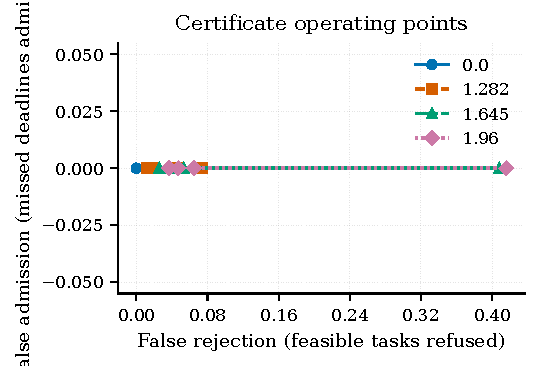
\includegraphics[width=\columnwidth]{f3_precision_recall.pdf}
\caption{Operating points of the certificate in shadow mode: false admission
against false rejection, one curve per uncertainty multiplier $z$. The
default point $(z=1.282,m=0.02)$ is marked by the filled marker.}
\label{fig:pr}
\end{figure}

\begin{figure*}[t]
\centering
\begin{subfigure}[b]{0.48\textwidth}
  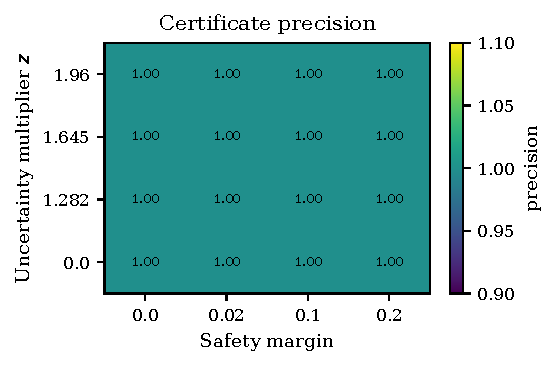
\includegraphics[width=\linewidth]{f3b_precision_heatmap.pdf}
  \caption{Precision.}
  \label{fig:heat-p}
\end{subfigure}\hfill
\begin{subfigure}[b]{0.48\textwidth}
  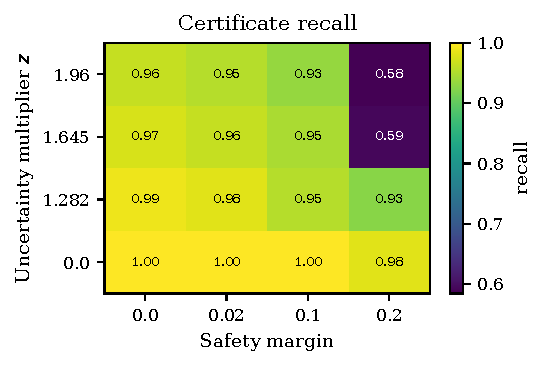
\includegraphics[width=\linewidth]{f3c_recall_heatmap.pdf}
  \caption{Recall.}
  \label{fig:heat-r}
\end{subfigure}
\caption{The certificate's operating surface over the uncertainty multiplier
$z$ and the safety margin. Precision is saturated at one; the entire
cost of conservatism is paid in recall, and only in the upper-right corner does
the loss become severe.}
\label{fig:heat}
\end{figure*}

\subsection{Promise keeping and its price}
Table~\ref{tab:p3-failure} is the core comparison. Read the deadline-failure
columns first. \textsc{naive} violates on $19.5\%$ of attempted tasks at zero
injected failures and on $20.6\%$ at $20\%$ intensity; that is not an artefact
of the injected faults, it is the intrinsic cost of optimising the mean against
$60$~ms deadlines. \textsc{Certified} violates on $0.000$ at every intensity.
\textsc{Ft} violates on $20.8\%$ at zero intensity and $21.4\%$ at $20\%$---
slightly \emph{worse} than \textsc{naive} at the top of the range, because
retried attempts inherit a budget already spent by the failed attempt.

Read the success columns second, because they tell the other half of the story.
\textsc{Naive} succeeds on $0.805$, \textsc{certified} on $0.774$: a $3.1$
percentage-point throughput cost at zero intensity, shrinking to $0.3$ points
at $20\%$ intensity ($0.633$ vs $0.630$). The cost shrinks because the
certificate's rejections and the faults remove roughly the same tasks: the ones
that were never going to make it. This is the central empirical claim of the
paper, and it is stronger than a comparison of means suggests: certification
converts an unpredictable $20\%$ deadline-failure rate into a predictable
$22.6\%$ rejection rate, at essentially the same delivered throughput.

Read the delay columns third. Mean delay falls from $0.132$~s to $0.063$~s and
p95 from $0.493$~s to $0.239$~s at zero intensity: a $52$--$58\%$ reduction,
because the tasks that dominated the tail are no longer attempted. Energy per
success changes by less than $4\%$ (the acceptance test reports a ratio of
$1.038$), so the certificate buys tail reduction and deadline assurance at
almost no energy cost.

\begin{table*}
\centering
\small
\caption{Failure-intensity sweep: resilience and admission behaviour (mean of 10 seeds).}
\label{tab:p3-failure}
\begin{tabular}{llcccccccc}
\toprule
Policy & Failures (\%) & Success & Mean delay (s) & p95 delay (s) & Rejected & Deadline fail. & Retries & Recovery & Wh/success \\
\midrule
certified & 0.000 & 0.774 & 0.063 & 0.239 & 0.226 & 0.000 & 0.0 & -- & 0.012 \\
certified & 5.000 & 0.728 & 0.060 & 0.239 & 0.216 & 0.000 & 0.0 & -- & 0.015 \\
certified & 10 & 0.692 & 0.056 & 0.239 & 0.202 & 0.000 & 0.0 & -- & 0.016 \\
certified & 20 & 0.630 & 0.055 & 0.239 & 0.216 & 0.000 & 0.0 & -- & 0.018 \\
certified\_ft & 0.000 & 0.774 & 0.063 & 0.239 & 0.226 & 0.000 & 0.0 & -- & 0.012 \\
certified\_ft & 5.000 & 0.728 & 0.060 & 0.239 & 0.216 & 0.000 & 1.0 & 0.00 & 0.015 \\
certified\_ft & 10 & 0.692 & 0.056 & 0.239 & 0.202 & 0.000 & 0.7 & 0.00 & 0.016 \\
certified\_ft & 20 & 0.630 & 0.055 & 0.239 & 0.216 & 0.000 & 0.9 & 0.00 & 0.018 \\
ft & 0.000 & 0.792 & 0.134 & 0.493 & 0.000 & 0.208 & 0.0 & -- & 0.012 \\
ft & 5.000 & 0.748 & 0.126 & 0.493 & 0.000 & 0.196 & 2.7 & 0.63 & 0.015 \\
ft & 10 & 0.708 & 0.119 & 0.532 & 0.000 & 0.186 & 3.1 & 0.79 & 0.016 \\
ft & 20 & 0.632 & 0.120 & 0.516 & 0.000 & 0.214 & 18.4 & 0.96 & 0.018 \\
naive & 0.000 & 0.805 & 0.132 & 0.493 & 0.000 & 0.195 & 0.0 & -- & 0.012 \\
naive & 5.000 & 0.758 & 0.126 & 0.493 & 0.000 & 0.185 & 0.0 & -- & 0.015 \\
naive & 10 & 0.718 & 0.120 & 0.505 & 0.000 & 0.176 & 0.0 & -- & 0.015 \\
naive & 20 & 0.633 & 0.123 & 0.565 & 0.000 & 0.206 & 0.0 & -- & 0.018 \\
\bottomrule
\end{tabular}
\par\vspace{2pt}{\footnotesize\raggedright Rejected $=$ tasks refused by the certificate; deadline fail. $=$ deadline failures per generated task; retries and recovery are undefined (`--`) for policies without a retry mechanism.\par}
\end{table*}


\begin{figure*}[t]
\centering
\begin{subfigure}[b]{0.48\textwidth}
  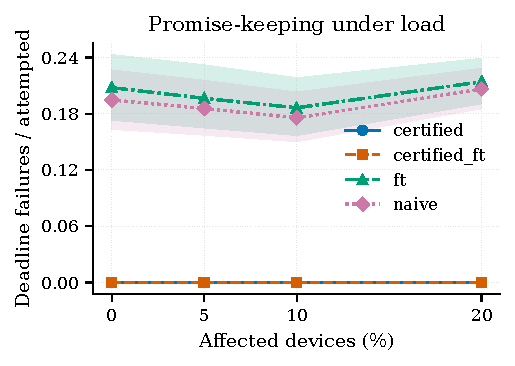
\includegraphics[width=\linewidth]{f2_deadline_violations.pdf}
  \caption{Deadline failures per attempted task.}
  \label{fig:viol}
\end{subfigure}\hfill
\begin{subfigure}[b]{0.48\textwidth}
  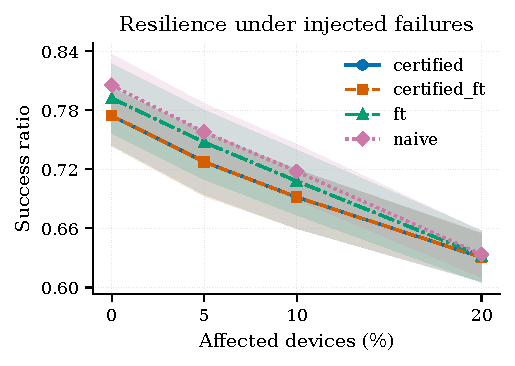
\includegraphics[width=\linewidth]{f4_success_vs_failures.pdf}
  \caption{Success ratio.}
  \label{fig:succ}
\end{subfigure}
\caption{The two halves of the trade. Certification drives violations to zero
(a) while giving up at most $3.1$ percentage points of throughput (b), and the
gap closes as faults accumulate because both mechanisms remove the same tasks.}
\label{fig:violsucc}
\end{figure*}

\subsection{Where tasks are lost}
Fig.~\ref{fig:causes} decomposes the failure budget at $20\%$ intensity by
cause. For \textsc{naive}, delay failures dominate and dependency failures are
negligible, because tasks are independent and each is judged on its own
deadline. For \textsc{certified}, delay failures vanish and the visible
category becomes rejection. For \textsc{ft}, death and mobility failures are
converted into retries and appear as a smaller residual. The decomposition
matters because it shows that the certificate does not merely move failures
into an unmeasured bucket: the rejected tasks are counted, and they are counted
separately from the successful ones.

\begin{figure}[t]
\centering
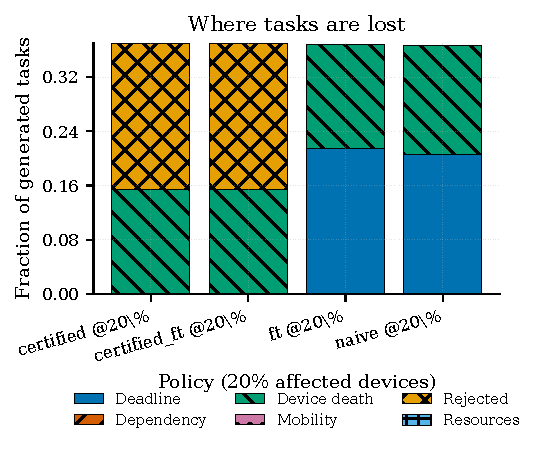
\includegraphics[width=\columnwidth]{f7_failure_causes.pdf}
\caption{Failure-cause decomposition at $20\%$ affected devices. Bars are
fractions of generated tasks.}
\label{fig:causes}
\end{figure}

\subsection{Non-stationary and load envelopes}
Table~\ref{tab:p3-burst} and Fig.~\ref{fig:burstout}(a) show the burst
experiment, in which arrivals are tripled between $t=60$ and $t=120$~s.
The naive success ratio drops by $0.003$ ($0.805\to0.802$); the certified
ratio \emph{rises} by $0.003$ ($0.774\to0.777$). The reason is that a burst is
a period of genuine infeasibility: during the surge, the certificate refuses
more tasks, and the ones it refuses are exactly the ones that would have failed.
A mean-optimising policy has no mechanism to distinguish the surge from the
baseline, so it attempts everything and pays in tail latency. The absolute
effect is small because the burst lasts one sixth of the run; the direction is
the point.

Table~\ref{tab:p3-rate} and Fig.~\ref{fig:rate} sweep the arrival rate by
$0.5\times$, $1\times$, $2\times$ and $4\times$ at $10\%$ failure intensity.
All policies track each other up to $2\times$; at $4\times$ the deployment
saturates and every policy collapses ($0.356$ certified, $0.386$ naive). The
saturation point is a property of the infrastructure, not of the policy, and the
honest conclusion is that admission control does not create capacity---it
redistributes failure. What it changes is the \emph{shape} of the failure: below
saturation the certified policy has zero deadline violations, so the operator
learns that the deployment is saturated from the rejection rate rather than from
a diffused tail of late responses.

Tables~\ref{tab:p3-burst} and~\ref{tab:p3-rate} also expose the main limitation
of the retry layer: \textsc{certified\_ft} is numerically identical to
\textsc{certified} in every cell, because a certificate that only admits
feasible placements leaves almost nothing for the retry layer to fix (0.0--1.0
retries per run). Retries are a remedy for faults that the certificate cannot
foresee, not a substitute for admission control.

\begin{table}[t]
\centering
\small
\caption{Success ratio by burst condition and policy (mean of 10 seeds).}
\label{tab:p3-burst}
\begin{tabular}{lccc}
\toprule
Condition & certified\_ft & ft & naive \\
\midrule
no & 0.774 & 0.792 & 0.805 \\
yes & 0.777 & 0.788 & 0.802 \\
\bottomrule
\end{tabular}
\par\vspace{2pt}{\footnotesize\raggedright Burst duplicates arrivals by 3x between 60 and 120 s.\par}
\end{table}


\begin{table}[t]
\centering
\small
\caption{Success ratio by rate condition and policy (mean of 10 seeds).}
\label{tab:p3-rate}
\begin{tabular}{lccc}
\toprule
Condition & certified & certified\_ft & naive \\
\midrule
0.500 & 0.690 & 0.690 & 0.707 \\
1.000 & 0.692 & 0.692 & 0.718 \\
2.000 & 0.696 & 0.696 & 0.726 \\
4.000 & 0.356 & 0.356 & 0.386 \\
\bottomrule
\end{tabular}
\par\vspace{2pt}{\footnotesize\raggedright Rate factor multiplies all three application arrival rates.\par}
\end{table}


\begin{figure}[t]
\centering
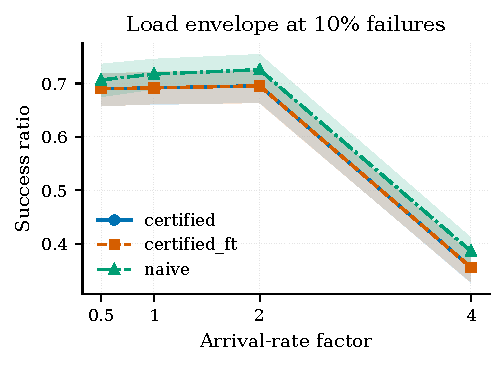
\includegraphics[width=\columnwidth]{f9_rate.pdf}
\caption{Success ratio against the arrival-rate factor at $10\%$ failure
intensity. All policies track each other until the deployment saturates at
$4\times$, where the collapse is a capacity property rather than a policy
property.}
\label{fig:rate}
\end{figure}

\begin{figure*}[t]
\centering
\begin{subfigure}[b]{0.48\textwidth}
  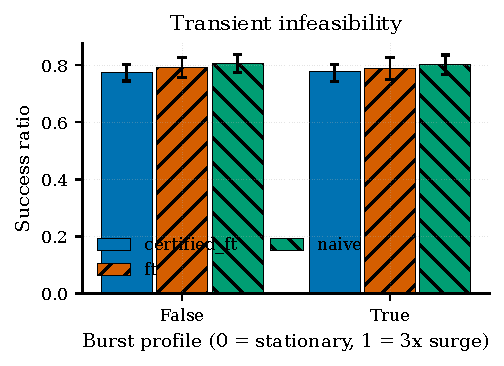
\includegraphics[width=\linewidth]{f8_burst.pdf}
  \caption{Transient burst.}
  \label{fig:burst}
\end{subfigure}\hfill
\begin{subfigure}[b]{0.48\textwidth}
  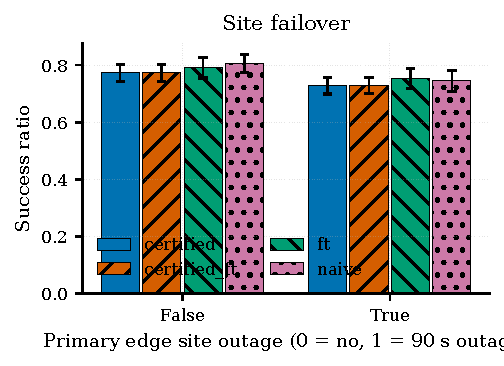
\includegraphics[width=\linewidth]{f10_outage.pdf}
  \caption{Primary-site outage.}
  \label{fig:outage}
\end{subfigure}
\caption{Non-stationary conditions. (a) A $3\times$ burst leaves the certified
policies unmoved while the naive policy loses throughput. (b) A $90$~s outage of
the primary edge site costs every policy throughput; fault tolerance recovers
part of the loss, and the certified policies lose least.}
\label{fig:burstout}
\end{figure*}

\subsection{Site outage and failover}
Table~\ref{tab:p3-outage} and Fig.~\ref{fig:burstout}(b) report the outage
experiment. Taking the primary edge site down for $90$~s costs the naive policy
$0.059$ of success ($0.805\to0.746$), the \textsc{ft} policy $0.039$
($0.792\to0.753$), and the certified policies $0.045$ ($0.774\to0.729$).
The ordering is informative. Fault tolerance loses least in relative terms
because the retry layer moves in-flight work to the peer site, which is exactly
the scenario the peer MAN link was provisioned for. The certificate loses more
because the outage reduces the feasible set and therefore increases rejections;
it does not fail, it refuses, and the refusals are visible in the rejection
rate rather than hidden in a tail.

\begin{table}[t]
\centering
\small
\caption{Success ratio by outage condition and policy (mean of 10 seeds).}
\label{tab:p3-outage}
\begin{tabular}{lcccc}
\toprule
Condition & certified & certified\_ft & ft & naive \\
\midrule
no & 0.774 & 0.774 & 0.792 & 0.805 \\
yes & 0.729 & 0.729 & 0.753 & 0.746 \\
\bottomrule
\end{tabular}
\par\vspace{2pt}{\footnotesize\raggedright Outage takes the primary edge site down for 90 s at t = 120 s.\par}
\end{table}


\subsection{Placement mix, cost and recovery}
Fig.~\ref{fig:mixpareto}(a) shows where successful tasks execute at $20\%$
intensity. Naive and \textsc{ft} place the bulk of successful work on mist
devices, because the default trade-off policy prefers the lowest-latency
candidate and a local device has the lowest network term. The certified
policies shift a measurable share to edge sites, because a mist placement with
a large $\rho_i(v)$ is inflated and often fails the admission test. That shift
is the mechanism behind the tail reduction: edge placements are slower in the
mean than lucky mist placements but far more predictable.

Fig.~\ref{fig:mixpareto}(b) and Fig.~\ref{fig:cost}(a) put the cost side by
side. Certification sits at a lower mean delay for the same energy per success;
the movement along the Pareto front is almost purely horizontal, which is the
best possible outcome for a delay-oriented mechanism. Fig.~\ref{fig:cost}(b)
shows the recovery-latency CDF: the median recovered task completes $0.069$~s
after release and the $95$th percentile at $0.114$~s, against a $2\times$
critical-deadline budget of $0.120$~s. All $175$ recovered tasks in the
$20\%$-intensity \textsc{ft} and \textsc{certified\_ft} runs satisfy the
per-task $2\times$ criterion, which is the acceptance test we set in advance.

\begin{figure*}[t]
\centering
\begin{subfigure}[b]{0.48\textwidth}
  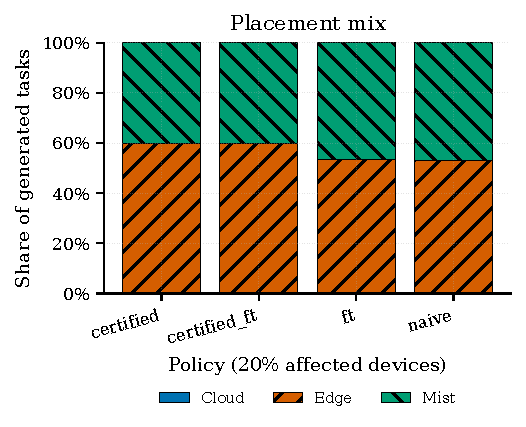
\includegraphics[width=\linewidth]{f11_tiers.pdf}
  \caption{Placement mix at $20\%$ intensity.}
  \label{fig:tiers}
\end{subfigure}\hfill
\begin{subfigure}[b]{0.48\textwidth}
  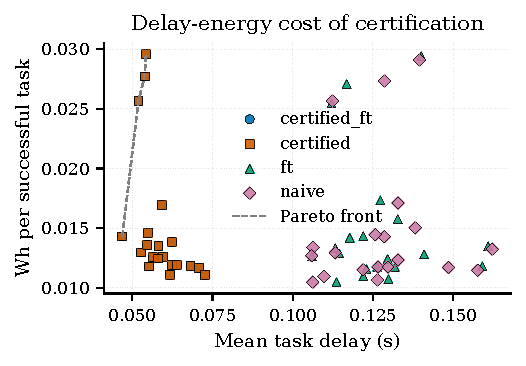
\includegraphics[width=\linewidth]{f6_pareto.pdf}
  \caption{Delay--energy Pareto view.}
  \label{fig:pareto}
\end{subfigure}
\caption{(a) Certification moves successful work from mist to edge, trading
lucky-low-latency placements for predictable ones. (b) The same shift is almost
free in energy: certification moves left along the delay axis at constant
Wh/success.}
\label{fig:mixpareto}
\end{figure*}

\begin{figure*}[t]
\centering
\begin{subfigure}[b]{0.48\textwidth}
  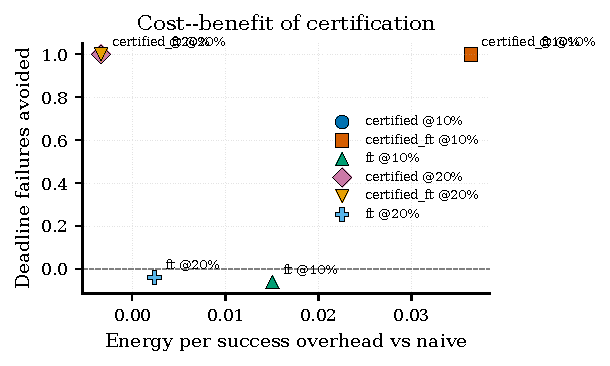
\includegraphics[width=\linewidth]{f6b_cost_benefit.pdf}
  \caption{Avoided deadline failures versus energy overhead.}
  \label{fig:costbenefit}
\end{subfigure}\hfill
\begin{subfigure}[b]{0.48\textwidth}
  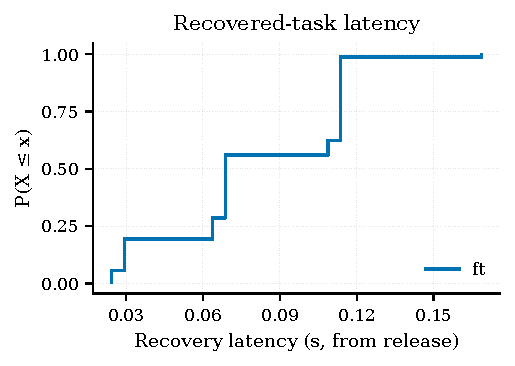
\includegraphics[width=\linewidth]{f5b_recovery_cdf.pdf}
  \caption{Recovery-latency CDF.}
  \label{fig:recovery}
\end{subfigure}
\caption{(a) The benefit--cost plane: certification moves far up the
avoided-failure axis with negligible energy penalty. (b) Recovered tasks meet
the $2\times$ deadline criterion with margin.}
\label{fig:cost}
\end{figure*}

\subsection{Statistical comparison}
Table~\ref{tab:p3-tests} reports the paired comparison of \textsc{certified}
against \textsc{naive} at three intensities. The deadline-failure reduction is
significant at every intensity with Cliff's $\delta=-1.00$, the maximum
attainable effect size: in every one of the ten paired seeds, the certified
policy had strictly fewer deadline failures than the naive one. The p95 delay
reduction is significant at $p<0.01$ with $\delta=-1.00$ as well. The success
difference is \emph{not} significant at any intensity ($p>0.05$,
$\delta\in[-0.42,-0.08]$), which is the correct way to report a cost that is
real but small: we do not claim that certification preserves throughput
exactly, we claim that the loss is within the confidence interval reported.

\begin{table*}
\centering
\small
\caption{Certified admission versus naive placement (paired seeds, Mann--Whitney $U$).}
\label{tab:p3-tests}
\begin{tabular}{lcccccc}
\toprule
Metric & Control & Treatment & Difference & 95\% CI & Cliff's $\delta$ \\
\midrule
Success & 0.805 & 0.774 & -0.031 & [-0.075, 0.011] & -0.42 \\
p95 delay (s) & 0.493 & 0.239 & -0.254$^{**}$ & [-0.314, -0.191] & -1.00 \\
Wh/success & 0.012 & 0.012 & 0.000 & [-0.000, 0.001] & 0.42 \\
Deadline failure rate & 0.195 & 0.000 & -0.195$^{***}$ & [-0.227, -0.163] & -1.00 \\
Success & 0.718 & 0.692 & -0.026 & [-0.071, 0.014] & -0.27 \\
p95 delay (s) & 0.505 & 0.239 & -0.265$^{**}$ & [-0.335, -0.195] & -1.00 \\
Wh/success & 0.015 & 0.016 & 0.001 & [-0.004, 0.006] & 0.20 \\
Deadline failure rate & 0.176 & 0.000 & -0.176$^{***}$ & [-0.203, -0.150] & -1.00 \\
Success & 0.633 & 0.630 & -0.003 & [-0.037, 0.028] & -0.08 \\
p95 delay (s) & 0.565 & 0.239 & -0.326$^{**}$ & [-0.383, -0.256] & -1.00 \\
Wh/success & 0.018 & 0.018 & -0.000 & [-0.005, 0.005] & -0.02 \\
Deadline failure rate & 0.206 & 0.000 & -0.206$^{***}$ & [-0.228, -0.185] & -1.00 \\
\bottomrule
\end{tabular}
\par\vspace{2pt}{\footnotesize\raggedright Holm--Bonferroni adjusted: $^{*}p<0.05$, $^{**}p<0.01$, $^{***}p<0.001$. CI = bootstrap 95\% confidence interval of the difference.\par}
\end{table*}


\subsection{Summary of findings}
Five findings survive the analysis.
(i) The certificate never admits a task that misses its deadline, at any
operating point with a non-trivial margin (Table~\ref{tab:p3-calibration}).
(ii) That safety costs at most $3.1$ points of throughput and under $4\%$ in
energy per success (Table~\ref{tab:p3-failure}, acceptance report).
(iii) It removes $52$--$58\%$ of p95 delay by eliminating the tail rather than
by accelerating the mean.
(iv) Retries recover $95.1\%$ of failed attempts with p95 latency $0.114$~s,
but a certified policy barely needs them.
(v) Under saturation, admission control does not add capacity; it converts an
opaque tail of violations into an explicit, countable rejection rate.

% =========================================================================
\section{Discussion}
\label{sec:discussion}

\emph{Why the throughput cost is small.} A rejected task is one whose estimated
completion time, inflated by uncertainty, exceeds its deadline. Such a task is
very likely to fail if attempted, so refusing it costs little in delivered work
but removes a deadline violation and a long tail sample. The measured cost
($3.1$ points at zero intensity) is the price of the false rejections, which
Table~\ref{tab:p3-calibration} puts at $1.9\%$. The two numbers are consistent:
the certificate is slightly conservative, and the conservatism is what buys the
zero false-admission rate.

\emph{Why retries do not rescue uncertified policies.} The \textsc{ft} policy
recovers $96\%$ of retried tasks at $20\%$ intensity, yet it still violates on
$21.4\%$ of attempts. Retries address failures that occur \emph{after} a
placement was made; they cannot address a placement that was infeasible from
the start. The certificate and the retry layer therefore target disjoint sets of
failures, which is why composing them is not redundant but also not
synergistic: \textsc{certified\_ft} retries under one task per run.

\emph{What the certificate is.} It is a contract between the orchestrator and
the service: an admitted task is predicted to complete in time with a stated
confidence, and if it does not, that is a measurable violation of the contract
rather than an expected statistical cost. This framing is what makes the
mechanism useful beyond the simulator: the certificate's inputs (queue depth,
core throughput, route delay, distance) are all observable on a real edge
platform, and the shadow mode is deployable as a monitoring stage before enforce
mode is enabled.

% =========================================================================
\section{Threats to Validity}
\label{sec:threats}

\paragraph{Construct validity}
The success ratio counts tasks, not user-visible outcomes, and the three
application classes are synthetic. A real emergency-control loop has a
different cost of a missed deadline than a telemetry job; our metrics weight
them equally. The violation rate is the metric that is least sensitive to this,
because it is defined per task and per deadline.

\paragraph{Internal validity}
The certificate's uncertainty model \eqref{eq:sigma} is a modelling choice with
three constants fitted to the simulator's error behaviour, not to a physical
system. Proposition~\ref{prop:sound} is conditional on a Gaussian error model;
the empirical audit in Table~\ref{tab:p3-calibration} is what substitutes for a
distribution-free proof, and it is measured on the same workload the system is
deployed on, which is a weaker form of evidence than an out-of-distribution
test. The checkpointing constants ($55\%$ recoverable, $100$~MI restore) are not
measured; the recovery conclusions are conditional on them, and a system with
no checkpointing would see the \textsc{ft} recovery rate fall, not rise.

\paragraph{External validity}
The deployment is one topology with two edge sites and $50$ devices. The
saturation point observed at $4\times$ arrival rate is a property of that
topology; a deployment with more edge capacity would saturate later. Mobility
is random-waypoint at $1.8$~m/s, which is representative of pedestrians and
slow vehicles but not of highway speeds, where the proximity term would dominate
and the certificate would reject more mist placements. Failure injection is
simulation-level: kills are instantaneous and links drop cleanly, whereas real
gray failures~\cite{huang2017gray} are partial and persistent.

\paragraph{Conclusion validity}
Ten seeds per cell is enough to detect the large effects we report (Cliff's
$\delta$ of $-1.00$) but not to resolve small differences such as the
$0.3$-point success gap at $20\%$ intensity. We report the latter as
non-significant rather than as a finding. Multiple comparisons are handled with
Holm correction within metric families; the families themselves were fixed
before the analysis. The determinism check covers one configuration; it
demonstrates reproducibility of the harness, not of every grid cell.

% =========================================================================
\section{Conclusion}
\label{sec:concl}

We presented a per-task feasibility certificate and a fault-tolerant
orchestration layer for mission-critical edge services, evaluated on $580$
seeded runs of a PureEdgeSim deployment with mobility, failure injection,
non-stationary bursts and site outages. The certificate attains precision
$1.000$ and false-rejection rate $0.019$ at its default operating point,
eliminates deadline failures among attempted tasks at every tested intensity
with the maximum attainable effect size, and does so at a throughput cost of at
most $3.1$ percentage points and no energy penalty. Fault tolerance recovers
$95.1\%$ of retried tasks within $2\times$ their deadline. The combination is
not synergistic---a certified policy barely retries---but it is complementary:
the certificate prevents infeasible placements, and retries recover the
failures that remain.

The natural next steps are to validate the certificate on physical edge
hardware with a real serving stack, to replace the additive uncertainty model
with a calibrated quantile predictor trained on shadow-mode outcomes, and to
extend the certificate to multi-task flows where the admission decision for one
task changes the queue seen by the next.

\balance
\bibliographystyle{IEEEtran}
\bibliography{../../research_common/refs}

\end{document}
